\documentclass[11pt,letterpaper]{article}
\usepackage[utf8]{inputenc}
\usepackage[T1]{fontenc}
\usepackage{amsmath}
\usepackage{amsfonts}
\usepackage{amssymb}
\usepackage{graphicx}
\usepackage{IEEEtrantools}
\usepackage{float}
\author{Alan Freeman}
\title{GAN Gogh: Use of a GAN to Imitate the Style of Vincent Van Gogh}
\begin{document}
% TODO: citations go inside periods.  I think.  Look it up.
% data.gov uses dataset as a single word, so we will adhere to that for this document
	\maketitle
	\section{Introduction}
		\subsection{Background}
			A GAN (Generative Adversarial Network) is a type of artificial intelligence composed of two neural networks, first introduced by Goodfellow et al in 2014 \cite{NIPS2014_5ca3e9b1}.
			% It takes its name from the fact that it uses two networks in direct opposition to each other.
			One, refered to as the generator, tries to generate images that resemble the training data.
			The other, called the discriminator, attempts to determine whether any given image is from the original dataset.
			
			%why does it get better at detecting fakes and how does generator improve
			% you can exand here .  More detail is better.
			As the discriminator gets better at detecting fakes, the generator has to improve the quality of its images in order to go undetected.
			This feedback loop produces images that become progressively more similar to the original input.
			The specific architecture of GAN that we used in this research was a Deep Convolutional GAN, or DCGAN, introduced by Radford et al in 2015.\cite{radford2015unsupervised}
		\subsection{Motivation}
			By training our GAN on images of paintings by Vincent Van Gogh, we hope to learn what specific features make his artwork so immediately recognizable.
			Towards this purpose, we collected 211 images from the Van Gogh Museum's website for use in training.
			Furthermore, we hope to create a tool that others can use to easily train their own GANs on their own data.

	\section{How We Approached Our Goal}
	
	% TODO: Too abstract or not abstract enough.  
	% Either bring in the code blocks you are referencing with minted or listing package
	% or remove references from your text of specific code blocks.
	
		To accomplish our goals, we assembled a Jupyter notebook that trains a DCGAN on user-specified data.
		Large parts of our code come from the TorchGAN\cite{pal2019torchgan} project's tutorial examples.

		The first code block checks whether the environment in which the notebook is running has TorchGAN installed, and installs it if missing.
		This block is primarily included for interoperability with Google Colab, which does not have TorchGAN installed by default.
		The following block contains all of the import statements required for the rest of the code.

		The third block uses a class from the TorchVision package of Torch to set up the dataset that the GAN will be training on.
		Figuring out how to write the code for this block was quite time-consuming, and included multiple false starts.
		Our first attempt involved reading the files and converting them to NumPy arrays, then saving each array to a file.
		However, we then realized that this solution wasn't actually compatible with the TorchGAN code, so we started going through the documentation of the built-in datasets to figure out what we should subclass.
		Once we found the appropriate class, we began writing a custom dataset class that would allow the user to specify a directory, and from that, load all of the images in that directory as a dataset.
		We then learned that this was almost exactly the same usage and behavior as the already-existing ImageFolder class in the TorchVision package, so we switched to using that instead.

		Functionally, the block creates an ImageFolder object in memory from the directory provided.
		The images are scaled to the specified size, normalized, and, if specified, converted to grayscale.

		The fourth, fifth, sixth, seventh, and ninth blocks are all adapted from the TorchGAN tutorial.

		The eighth and tenth blocks allow the user to continue training a previously-created model.

	\section{How to Use Our Code}
		If no other instructions are provided for a block, it can be run without any changes.

		If you are running our code on Colab, be sure to either run the first block or manually install TorchGAN, as Colab doesn't have it installed by default.

		Before running the third block of code, you will need to change some settings.
		First, choose the size of the images.
		This number must be an exact power of 2, and no smaller than 16.
		Larger values have the potential to create more detailed images, but will increase the time it takes to train.
		Second, if the images you are using are in black and white, set the grayscale variable to "True".
		Finally, specify the folder that the images are in.
		Due to the way that Torch's code works, you will have to specify the folder that contains the folder you want.
		This may require making a new folder and moving your folder into it.

		Before running the eighth block, you can choose to override the number of epochs that the model will train for.
		More epochs will take longer, but allow the model to become more refined.
		You can always resume training from a saved model later on.

		The ninth block should only be used if you are creating a brand new model.
		To resume training a previous model, use the tenth block.

		The tenth block can be used to continue training.
		In the first line of the block, specify the path to an existing model.
		The default value is the location that the notebook uses to save checkpoints.
		It should always be the most recent model, as long as the number of epochs was divisible by five.
		If you are running the notebook on Colab, you will need to manually save and upload your .model files, as Colab clears user data between sessions.

	\section{Generation of Results}
		\subsection{Parameters Used}
			The primary parameter which we manipulated was the training dataset.
			The datasets that we used were as follows:
			\begin{enumerate}
				\item The MNIST dataset (60,000 images)
				\item The images that we collected from the Van Gogh Museum (211 images)
				\item The Van Gogh images collected by the CycleGAN researchers (400 images)
				\item The Monet images collected by the CycleGAN researchers (1,000 images)
				\item The Monet images collected by the CycleGAN researchers, converted to grayscale (1,000 images)
				\item The landscape images collected by Jones and Bonafilia\cite{otherGanGogh} (15,000 images)
			\end{enumerate}
			Another parameter was the resolution of the images.
			The order of the values in the following list correspond to the order of the datasets listed above.
			\begin{enumerate}
				\item 32 by 32 pixels
				\item 256 by 256 pixels
				\item 256 by 256 pixels
				\item 256 by 256 pixels
				\item 256 by 256 pixels
				\item both 64 by 64 pixels and 128 by 128 pixels
			\end{enumerate}
			All other parameters remained constant between models.
		\subsection{Results}
		%TODO: if possible expand on captions
			\subsubsection{Van Gogh Museum Dataset}
				This dataset was our first attempt at our goal.
				For the first thousand or so epochs of training, the model produced nothing but static, with occasional blue patches.\footnote{Each figure is composed of a grid of generated samples.}
				See figure \ref{fig:vgm:epoch537generator}.
				\begin{figure}
					\centering
					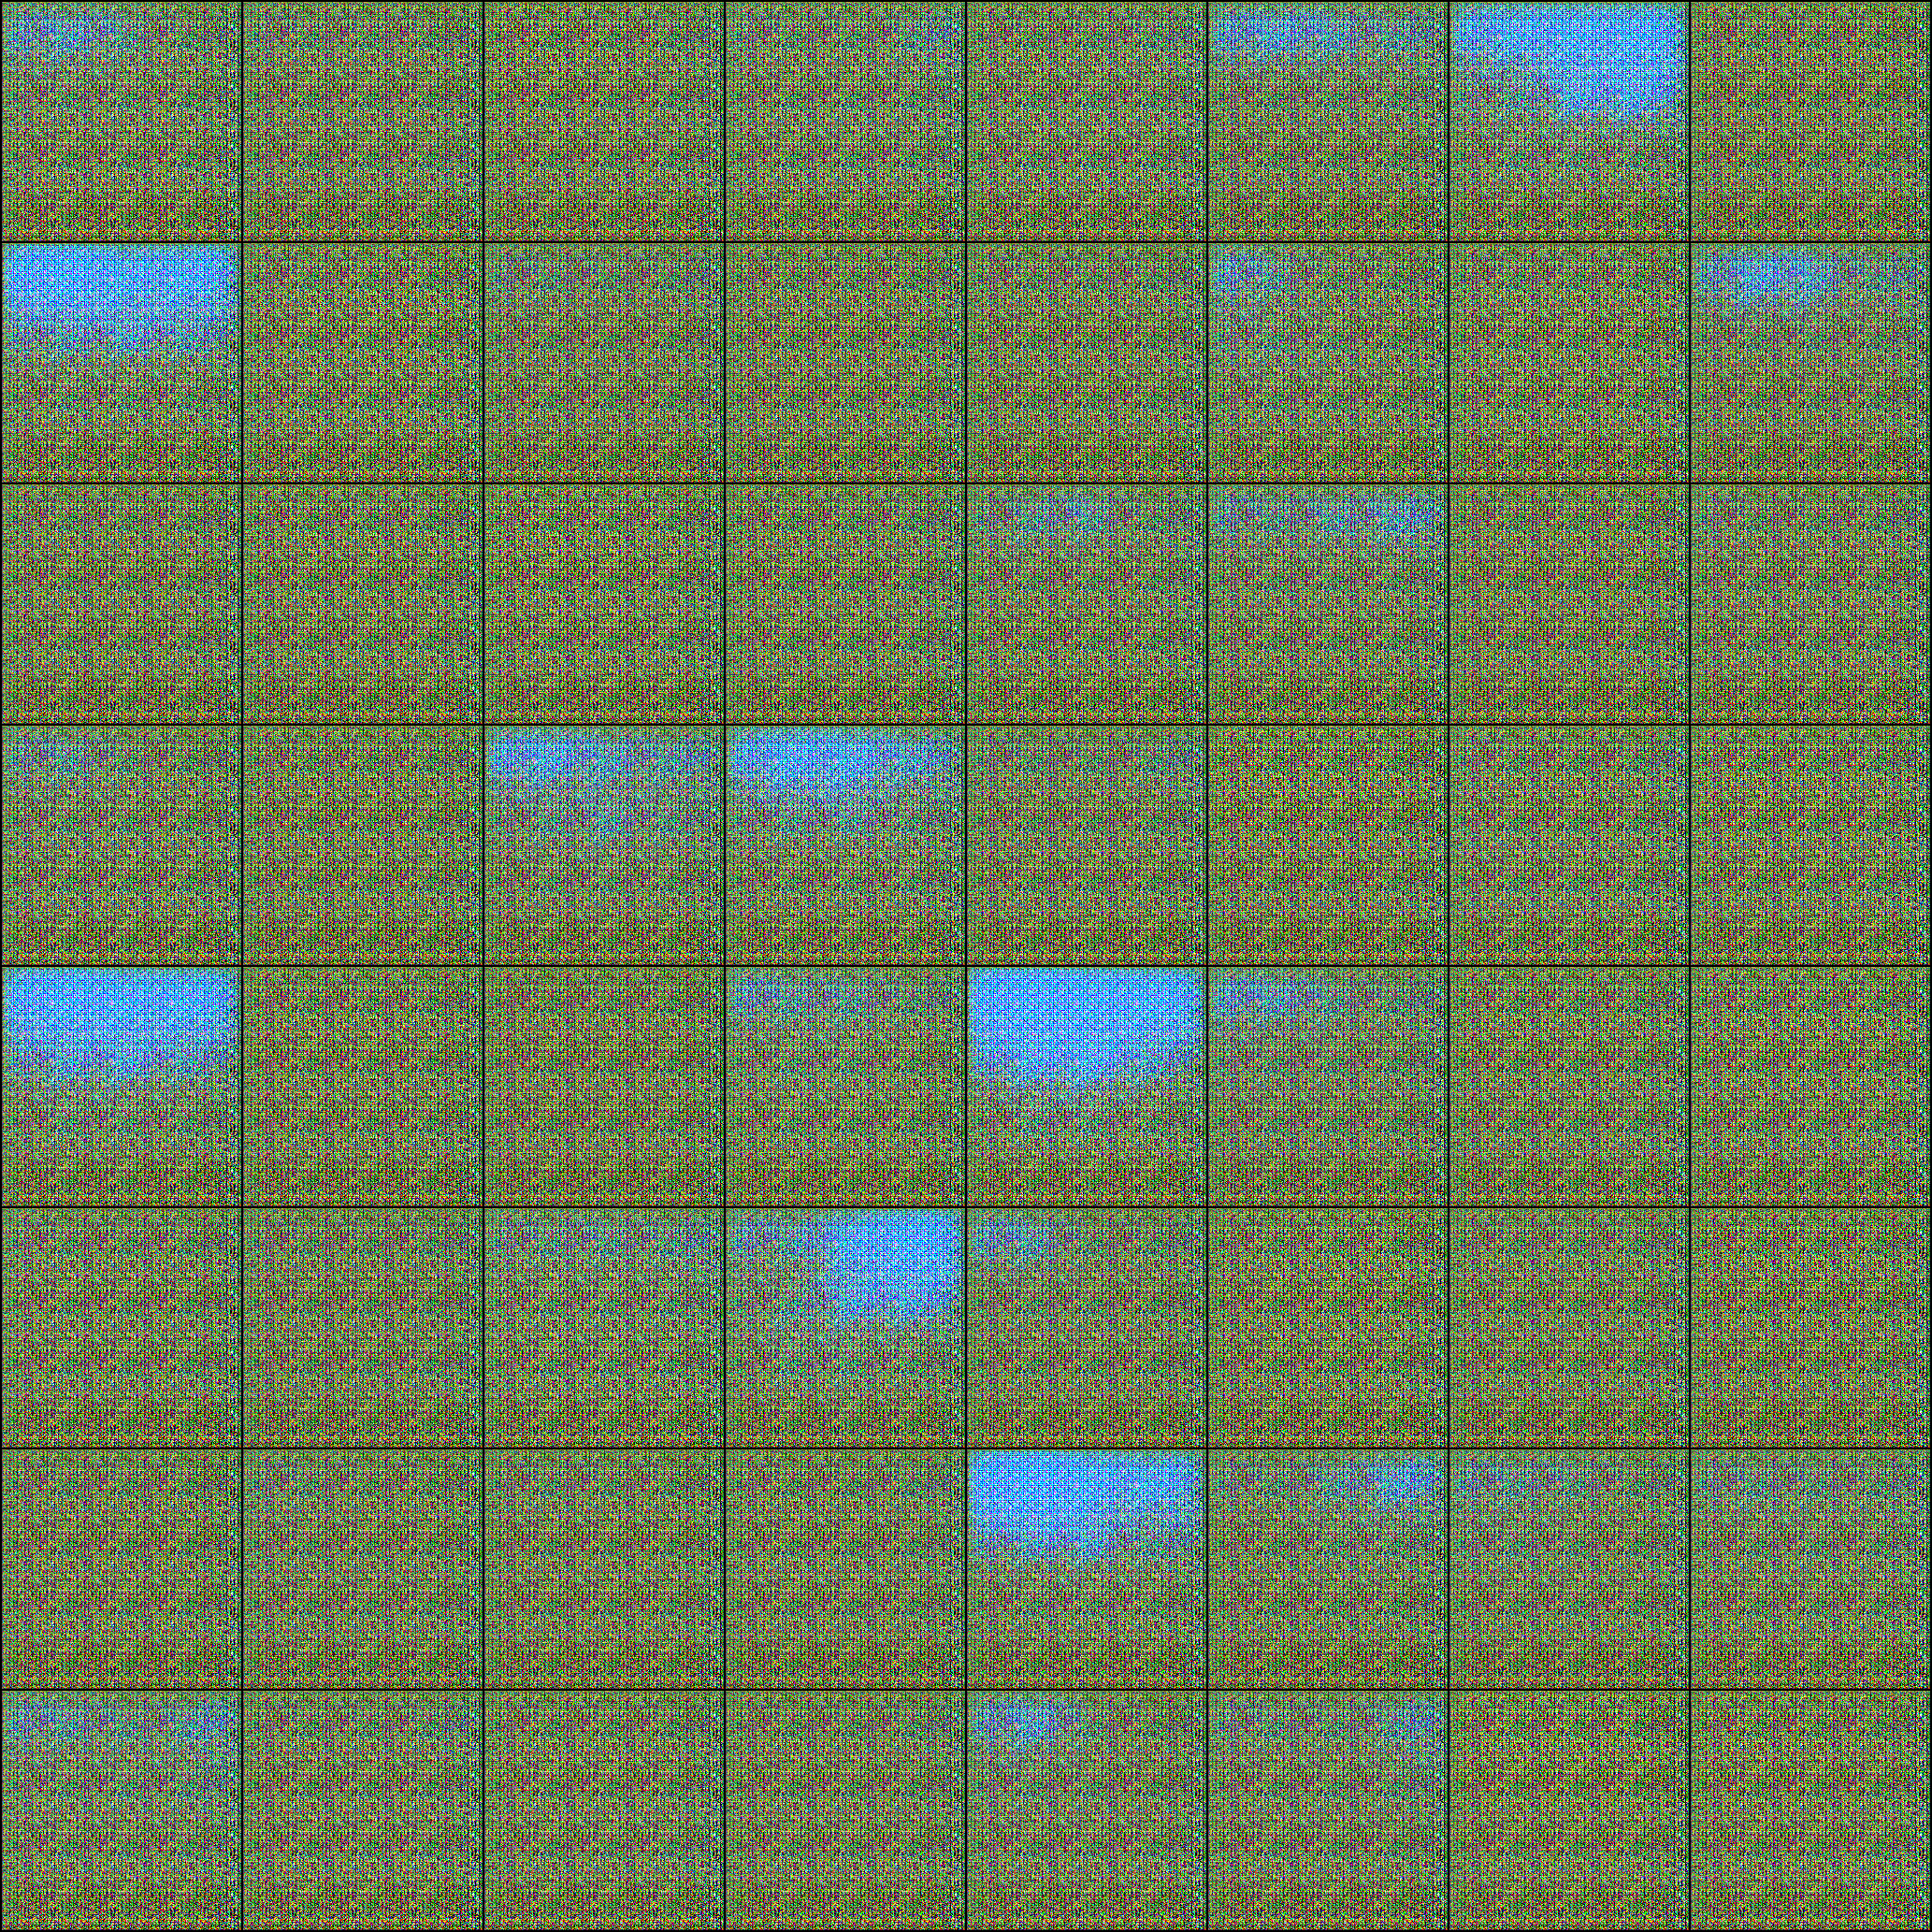
\includegraphics[width=1.0\linewidth]{past_attempts/van_gogh/DCGAN_2/images/epoch537_generator}
					\caption[Van Gogh Museum dataset, epoch 537]{Generated images from epoch 537. Note that the images are mostly random noise, with occasional splotches of color.}
					\label{fig:vgm:epoch537generator}
				\end{figure}

				This continues until around epoch 1087, at which point a grid begins to form.
				By epoch 1127, the grid is clearly visible.
				See figure \ref{fig:vgm:epoch1127generator}.
				\begin{figure}
					\centering
					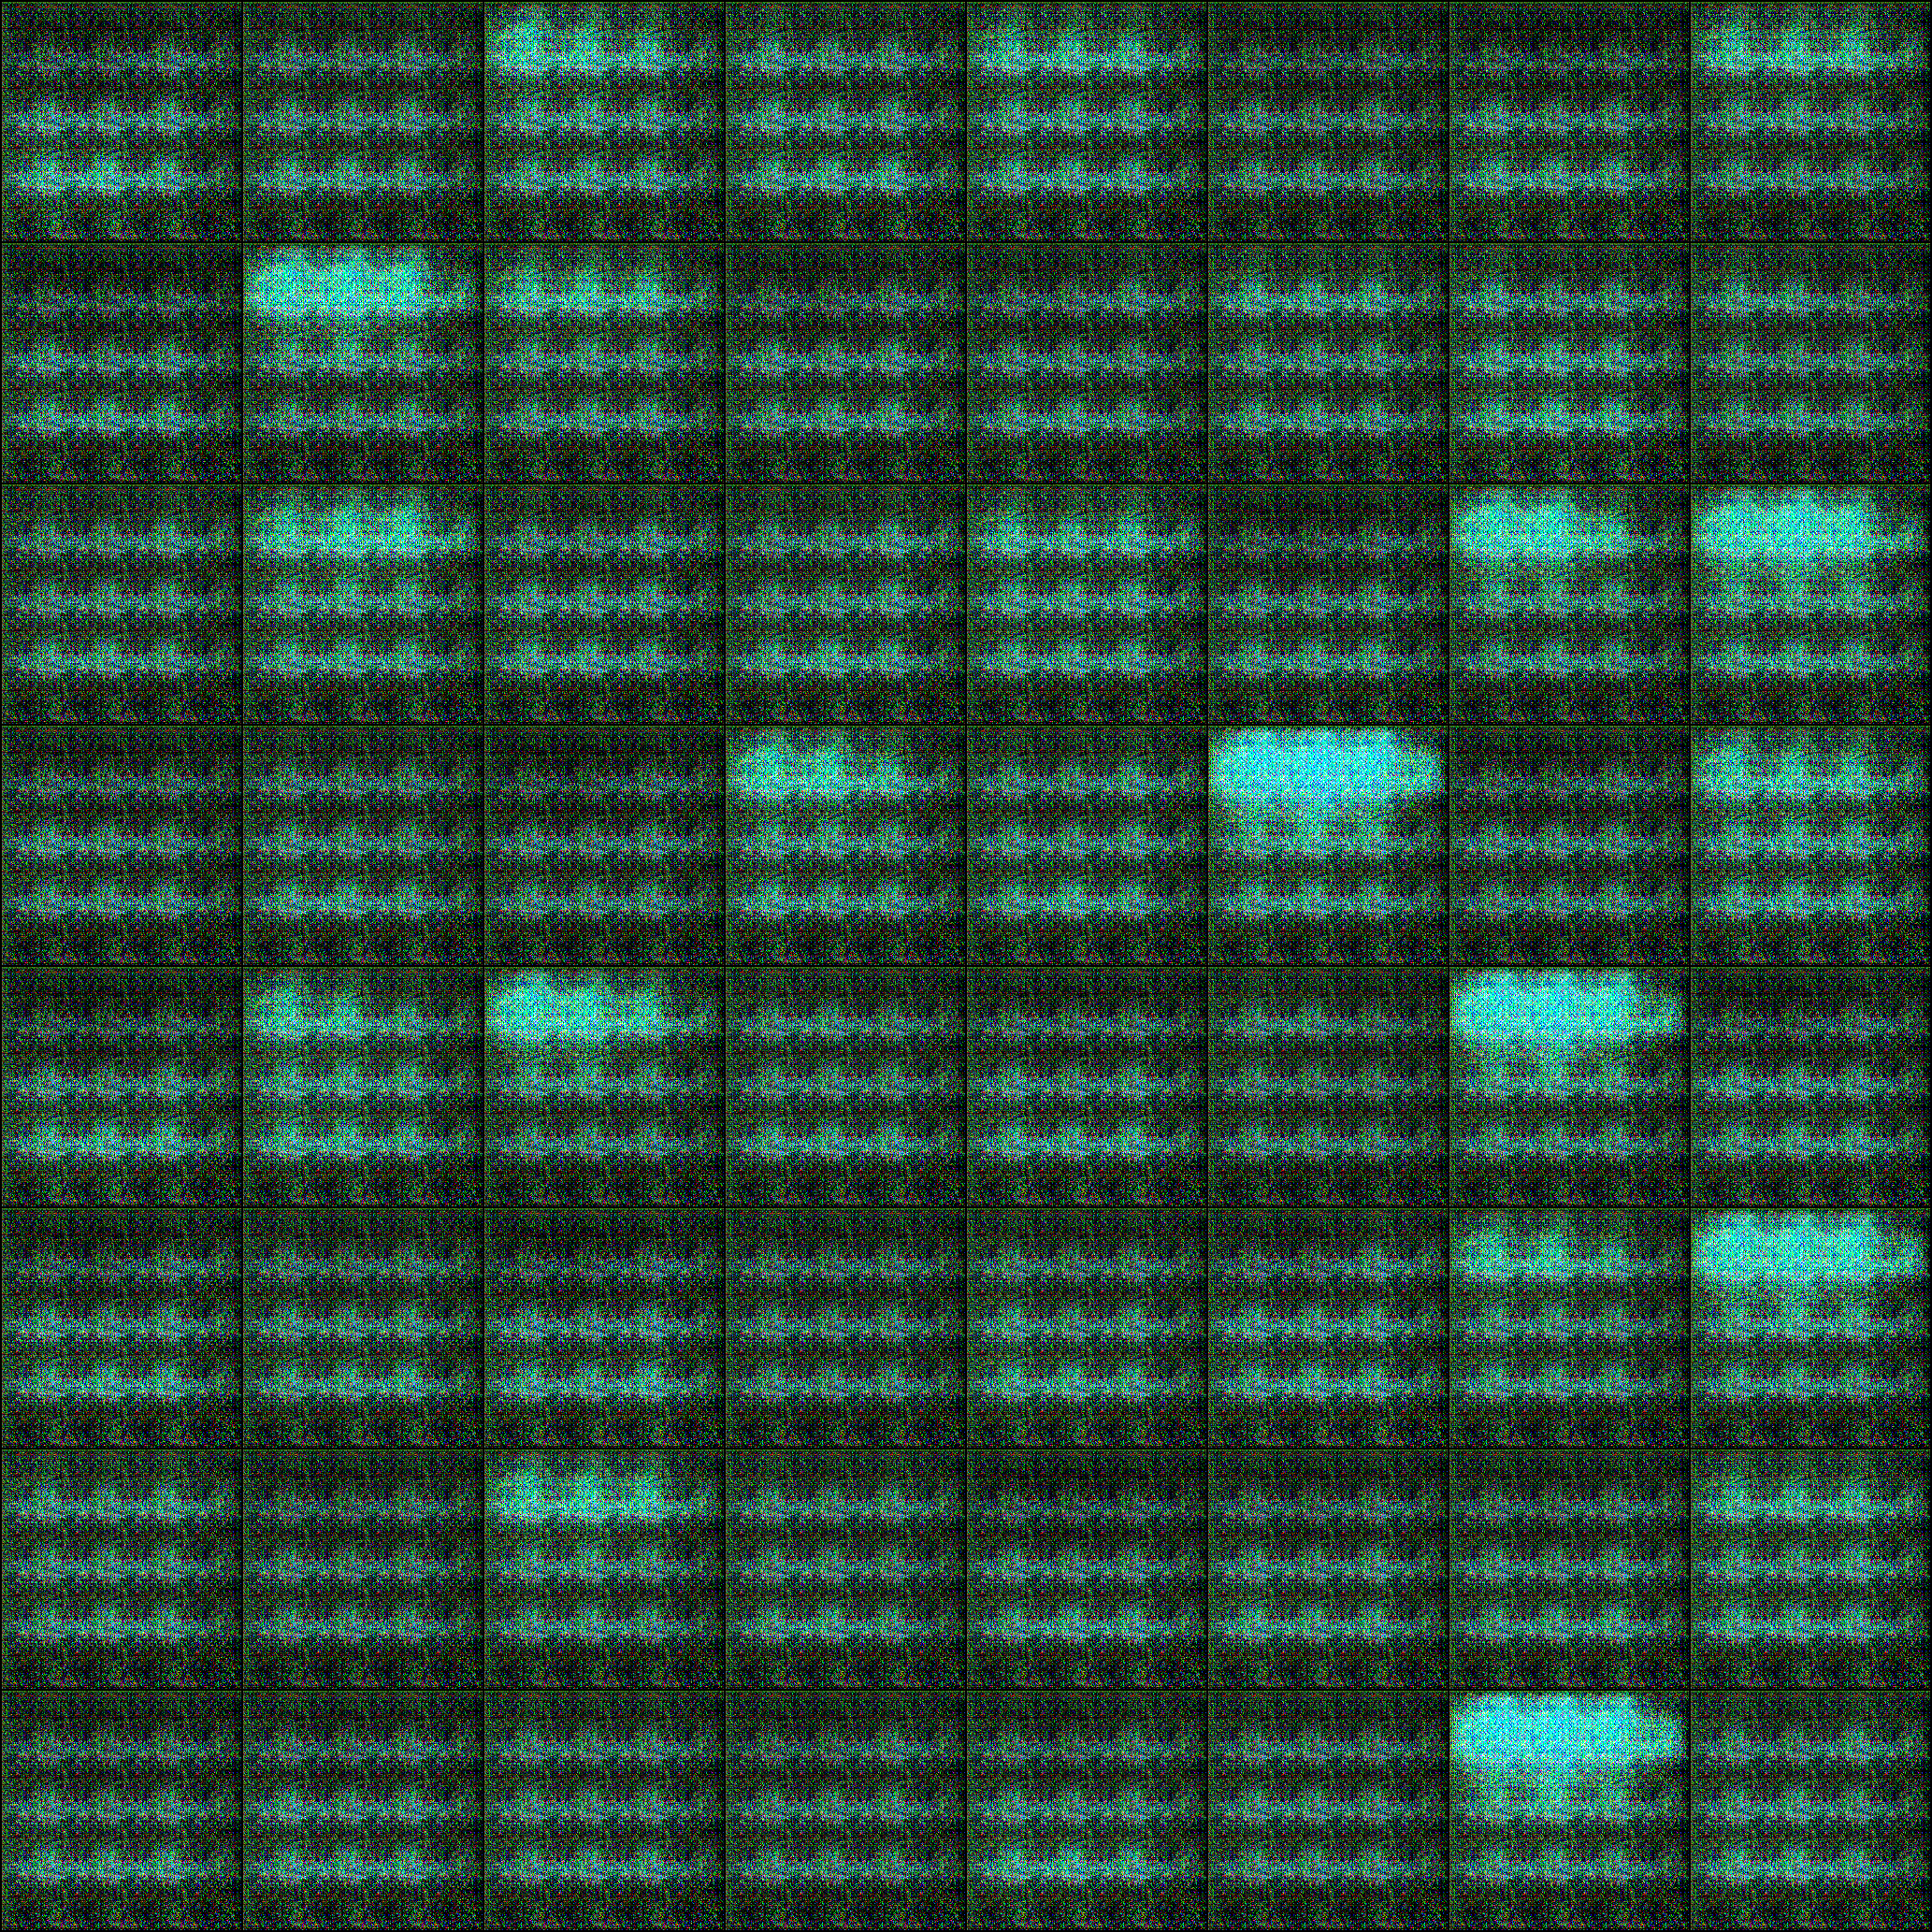
\includegraphics[width=1.0\linewidth]{past_attempts/van_gogh/DCGAN_2/images/epoch1127_generator}
					\caption[Van Gogh Museum dataset, epoch 1127]{Generated images from epoch 1127. Note the grid within the static of each image.}
					\label{fig:vgm:epoch1127generator}
				\end{figure}

				By epoch 1254, the grid has become a series of vertical lines.
				See figure \ref{fig:vgm:epoch1254generator}.
				\begin{figure}
					\centering
					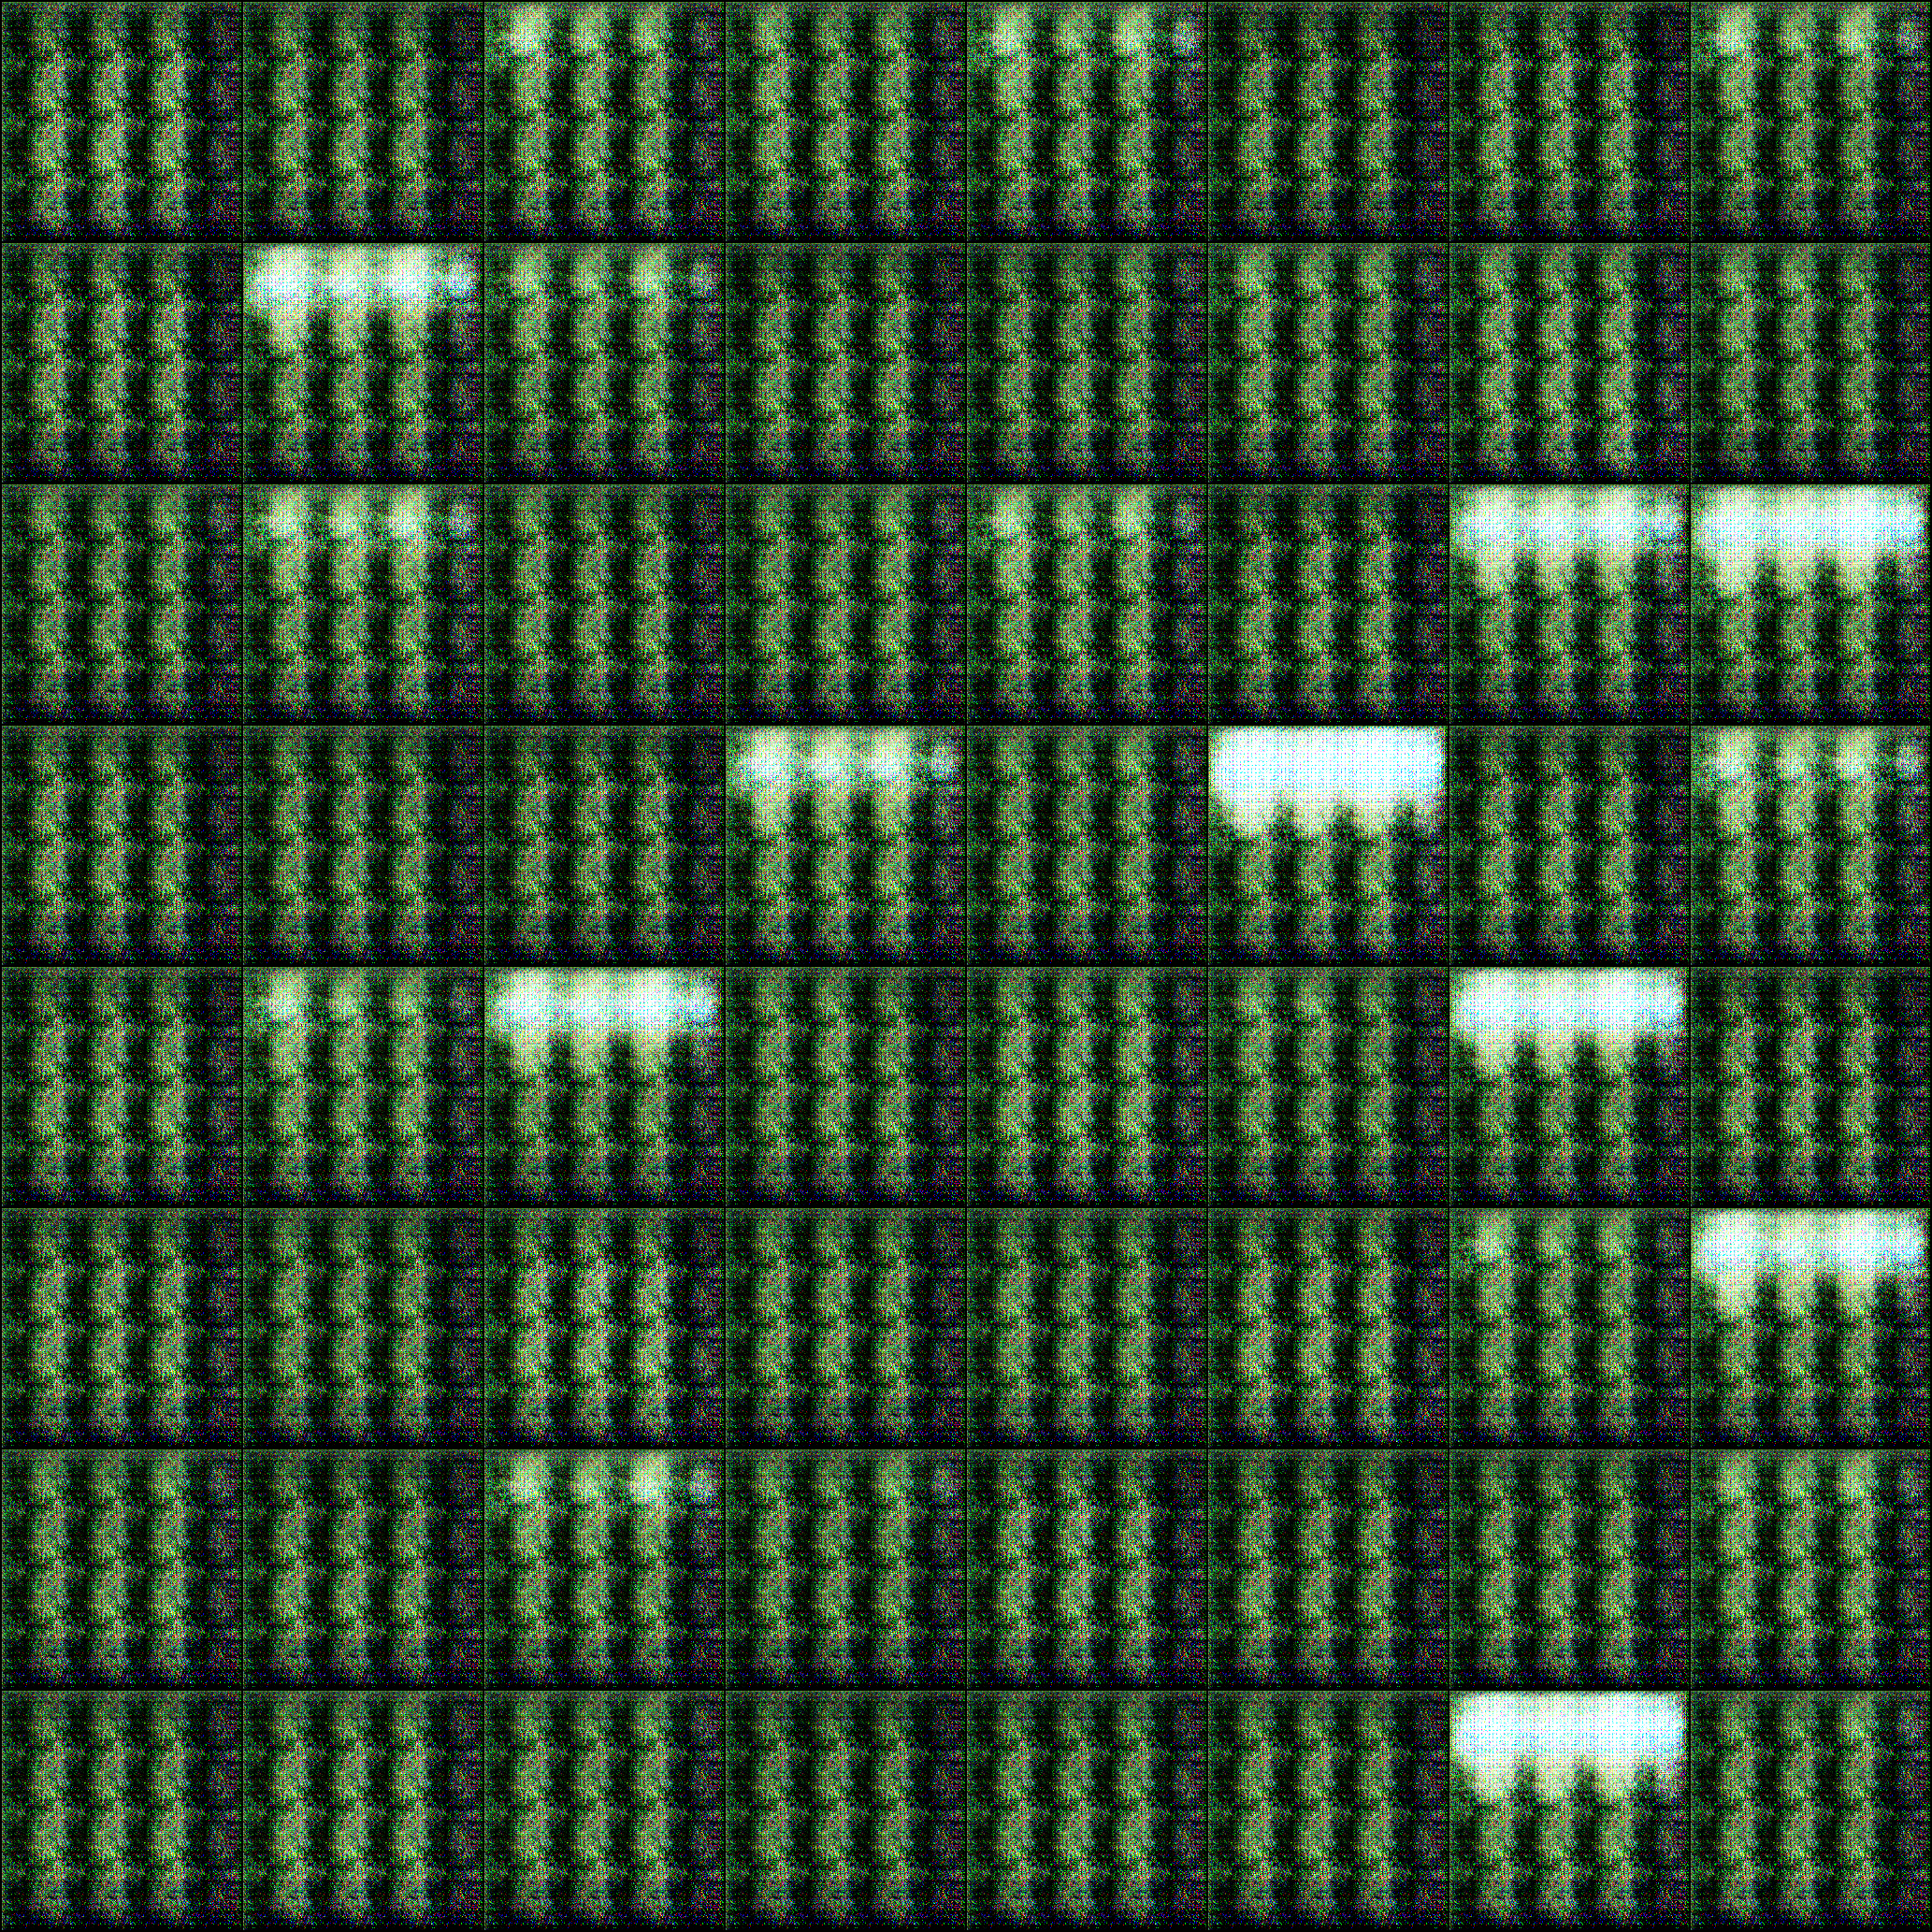
\includegraphics[width=1.0\linewidth]{past_attempts/van_gogh/DCGAN_2/images/epoch1254_generator}
					\caption[Van Gogh Museum dataset, epoch 1254]{Generated images from epoch 1254. Note the vertical lines that have formed.}
					\label{fig:vgm:epoch1254generator}
				\end{figure}

				By epoch 1406, the grid and lines are gone, and we are left with solid color with black borders.
				See figure \ref{fig:vgm:epoch1406generator}.
				It is worth noting that the black borders are due to a choice we made in preparing the images for training.
				In order to prevent image distortion due to stretching, we padded each image in this dataset, and this dataset alone, with extra pixels so that the width and height of each image was equal.
				That way, the scaling done would affect both dimensions equally, and therefore (in theory) preserve the image.
				Unfortunately, this did not have the intended effect.
				\begin{figure}
					\centering
					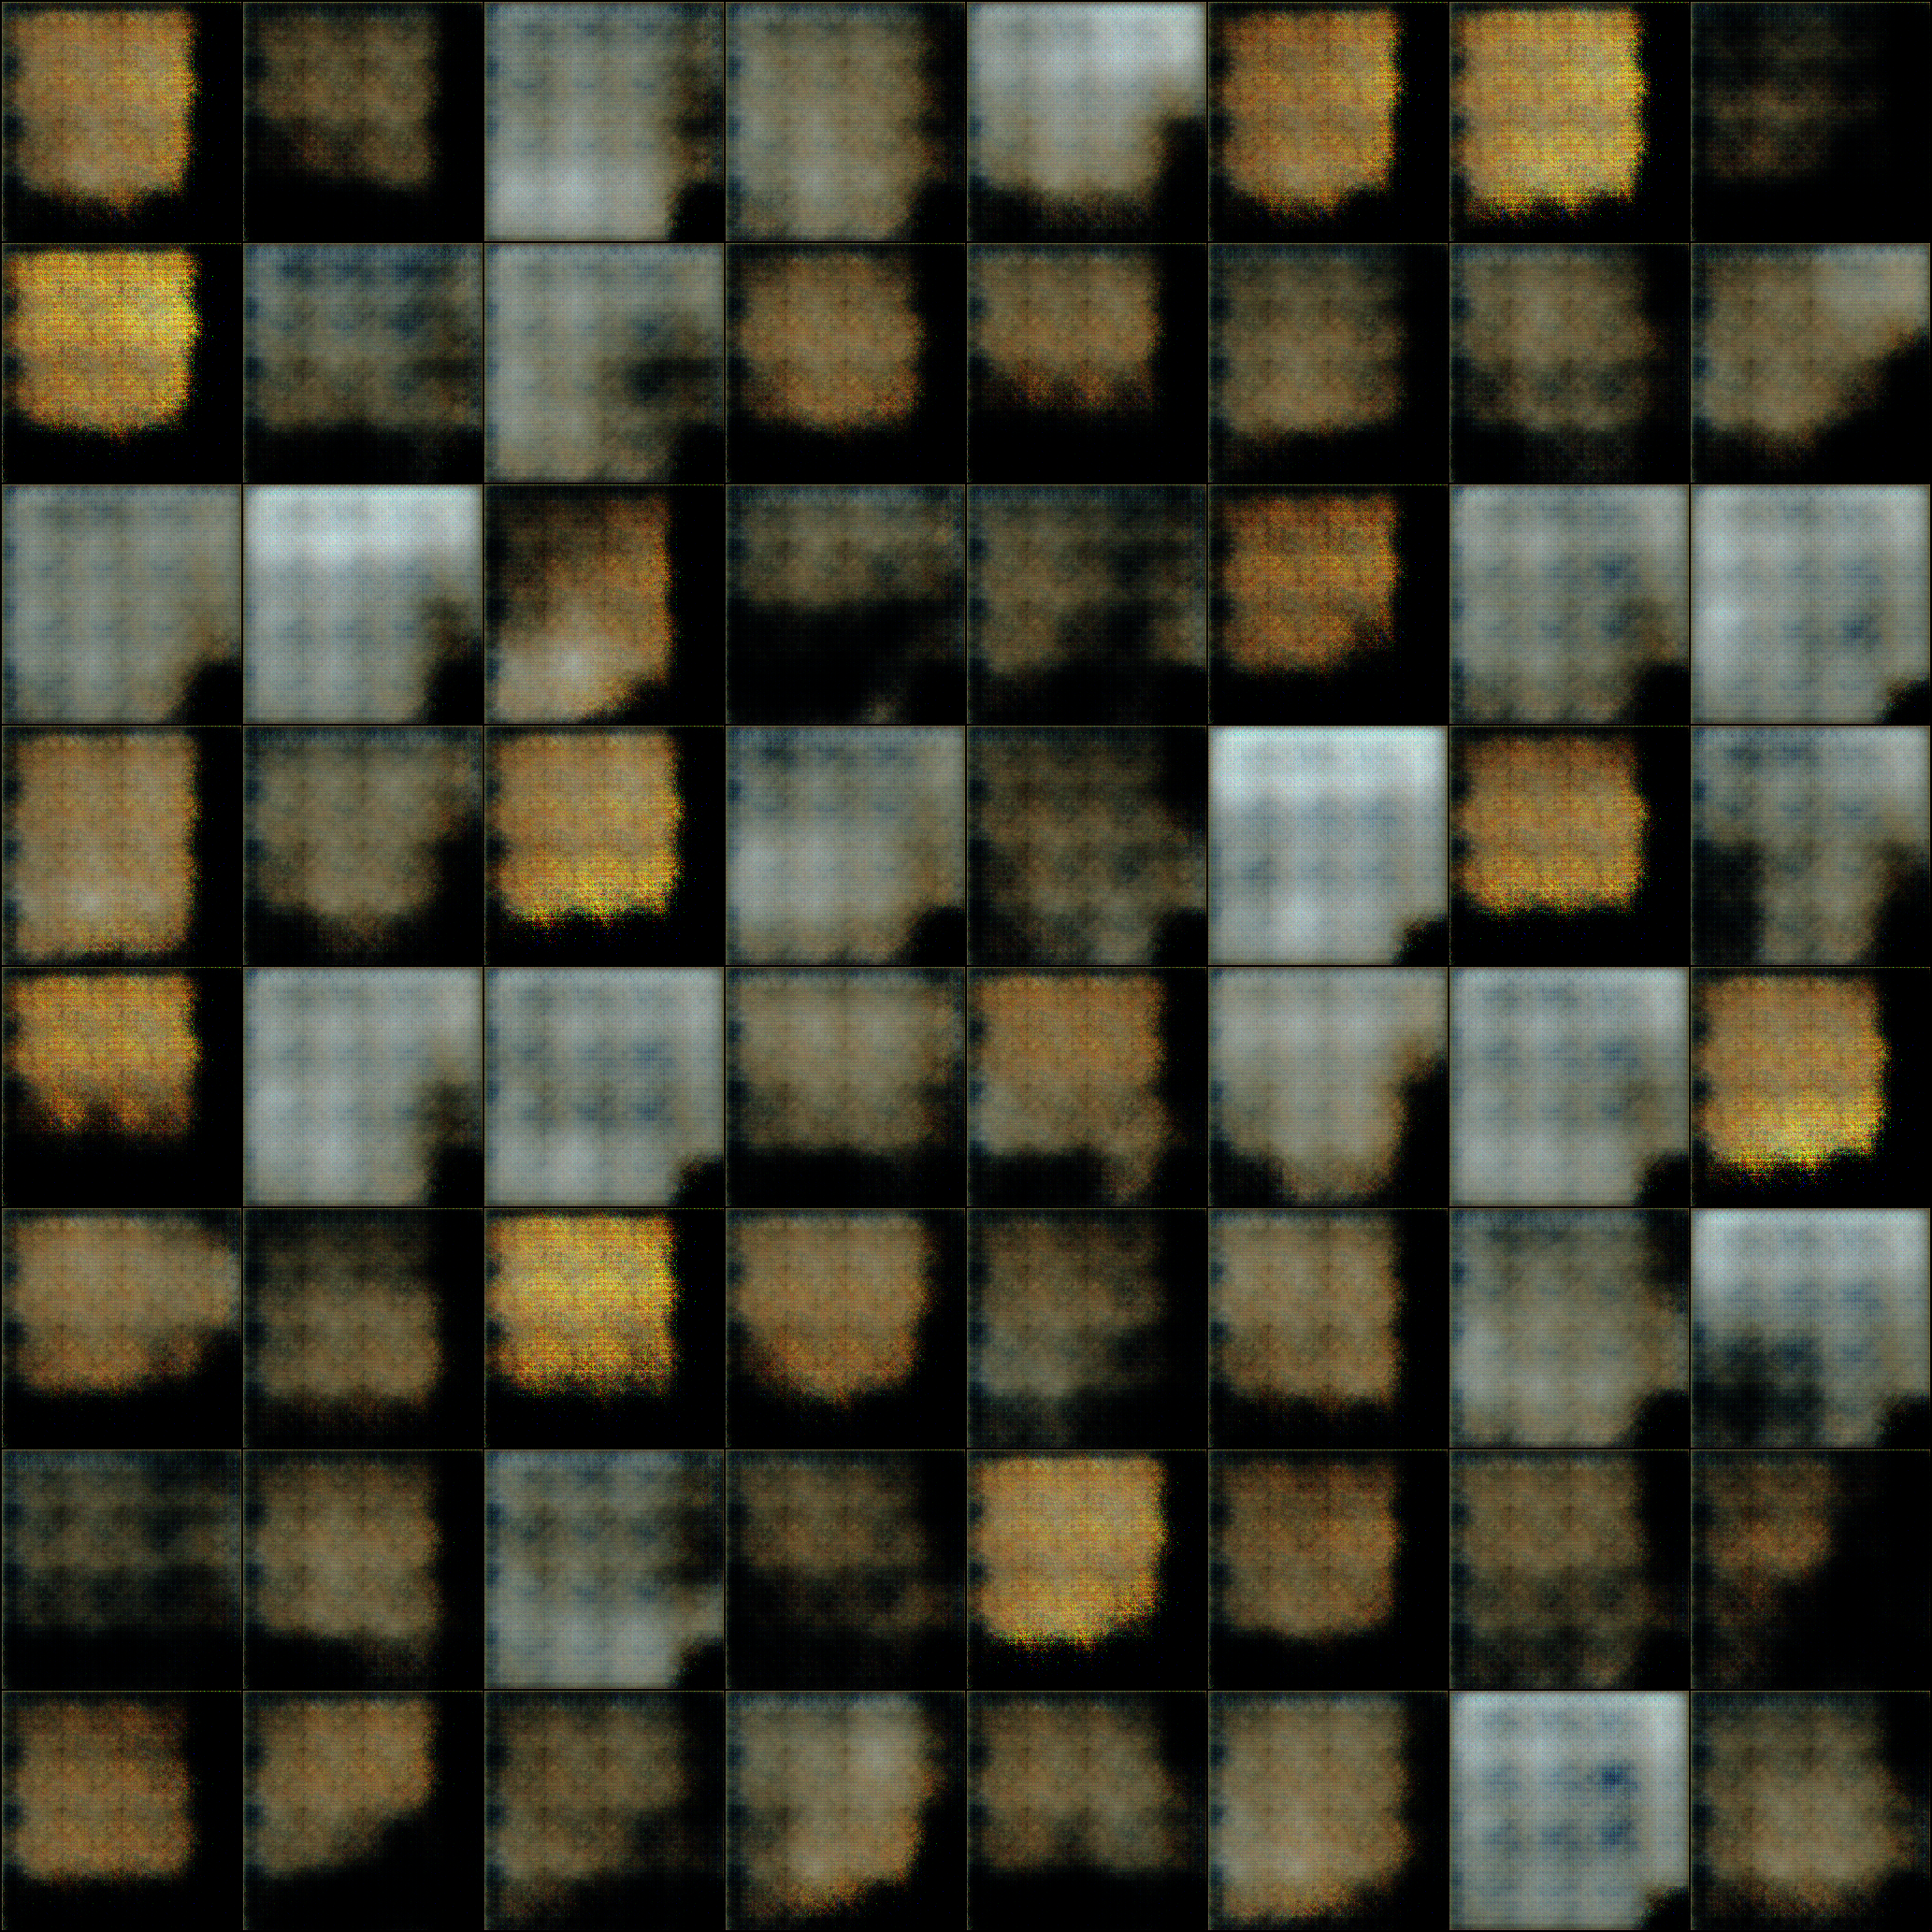
\includegraphics[width=1.0\linewidth]{past_attempts/van_gogh/DCGAN_2/images/epoch1406_generator}
					\caption[Van Gogh Museum dataset, epoch 1406]{Generated images from epoch 1406. Note the black bars.}
					\label{fig:vgm:epoch1406generator}
				\end{figure}

				By epoch 1531, a texture appears to form on the images.
				See figure \ref{fig:vgm:epoch1531generator}.
				\begin{figure}
					\centering
					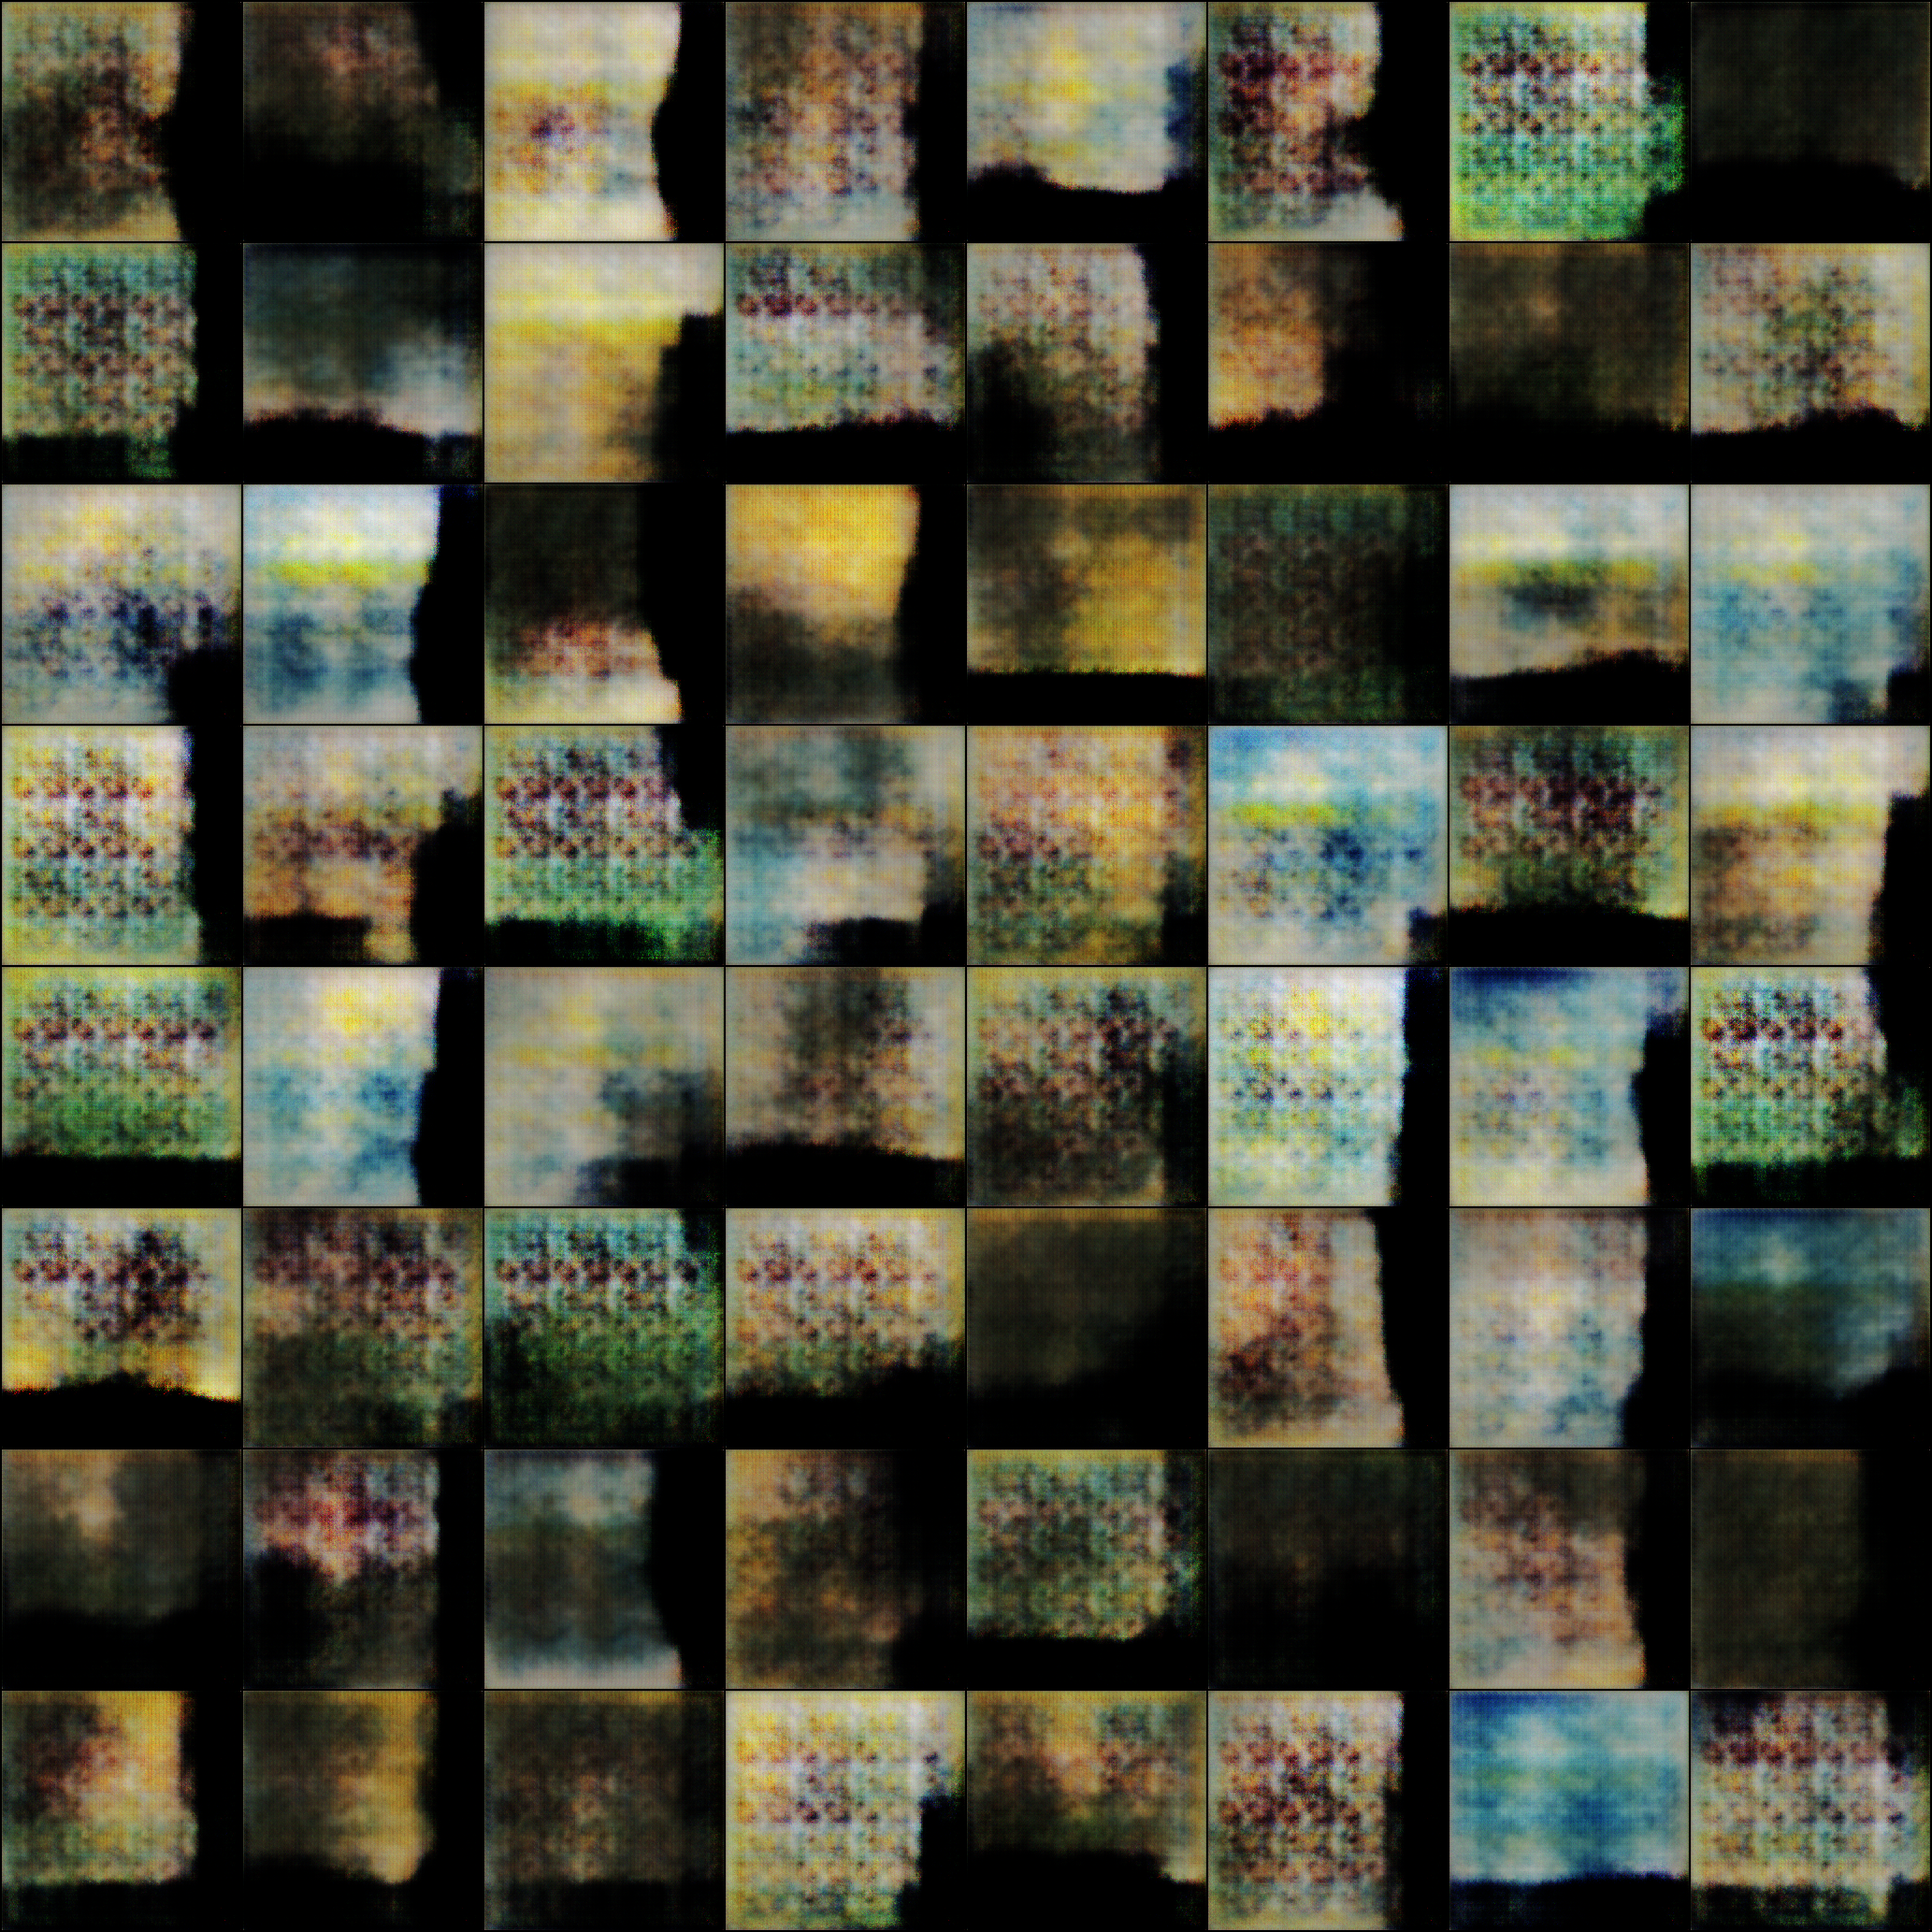
\includegraphics[width=1.0\linewidth]{past_attempts/van_gogh/DCGAN_2/images/epoch1531_generator}
					\caption[Van Gogh Museum dataset, epoch 1531]{Generated images from epoch 1531. Note the texture in the images.}
					\label{fig:vgm:epoch1531generator}
				\end{figure}

				At epoch 1702, the black bars are becoming more clearly defined.
				See figure \ref{fig:vgm:epoch1702generator}.
				\begin{figure}
					\centering
					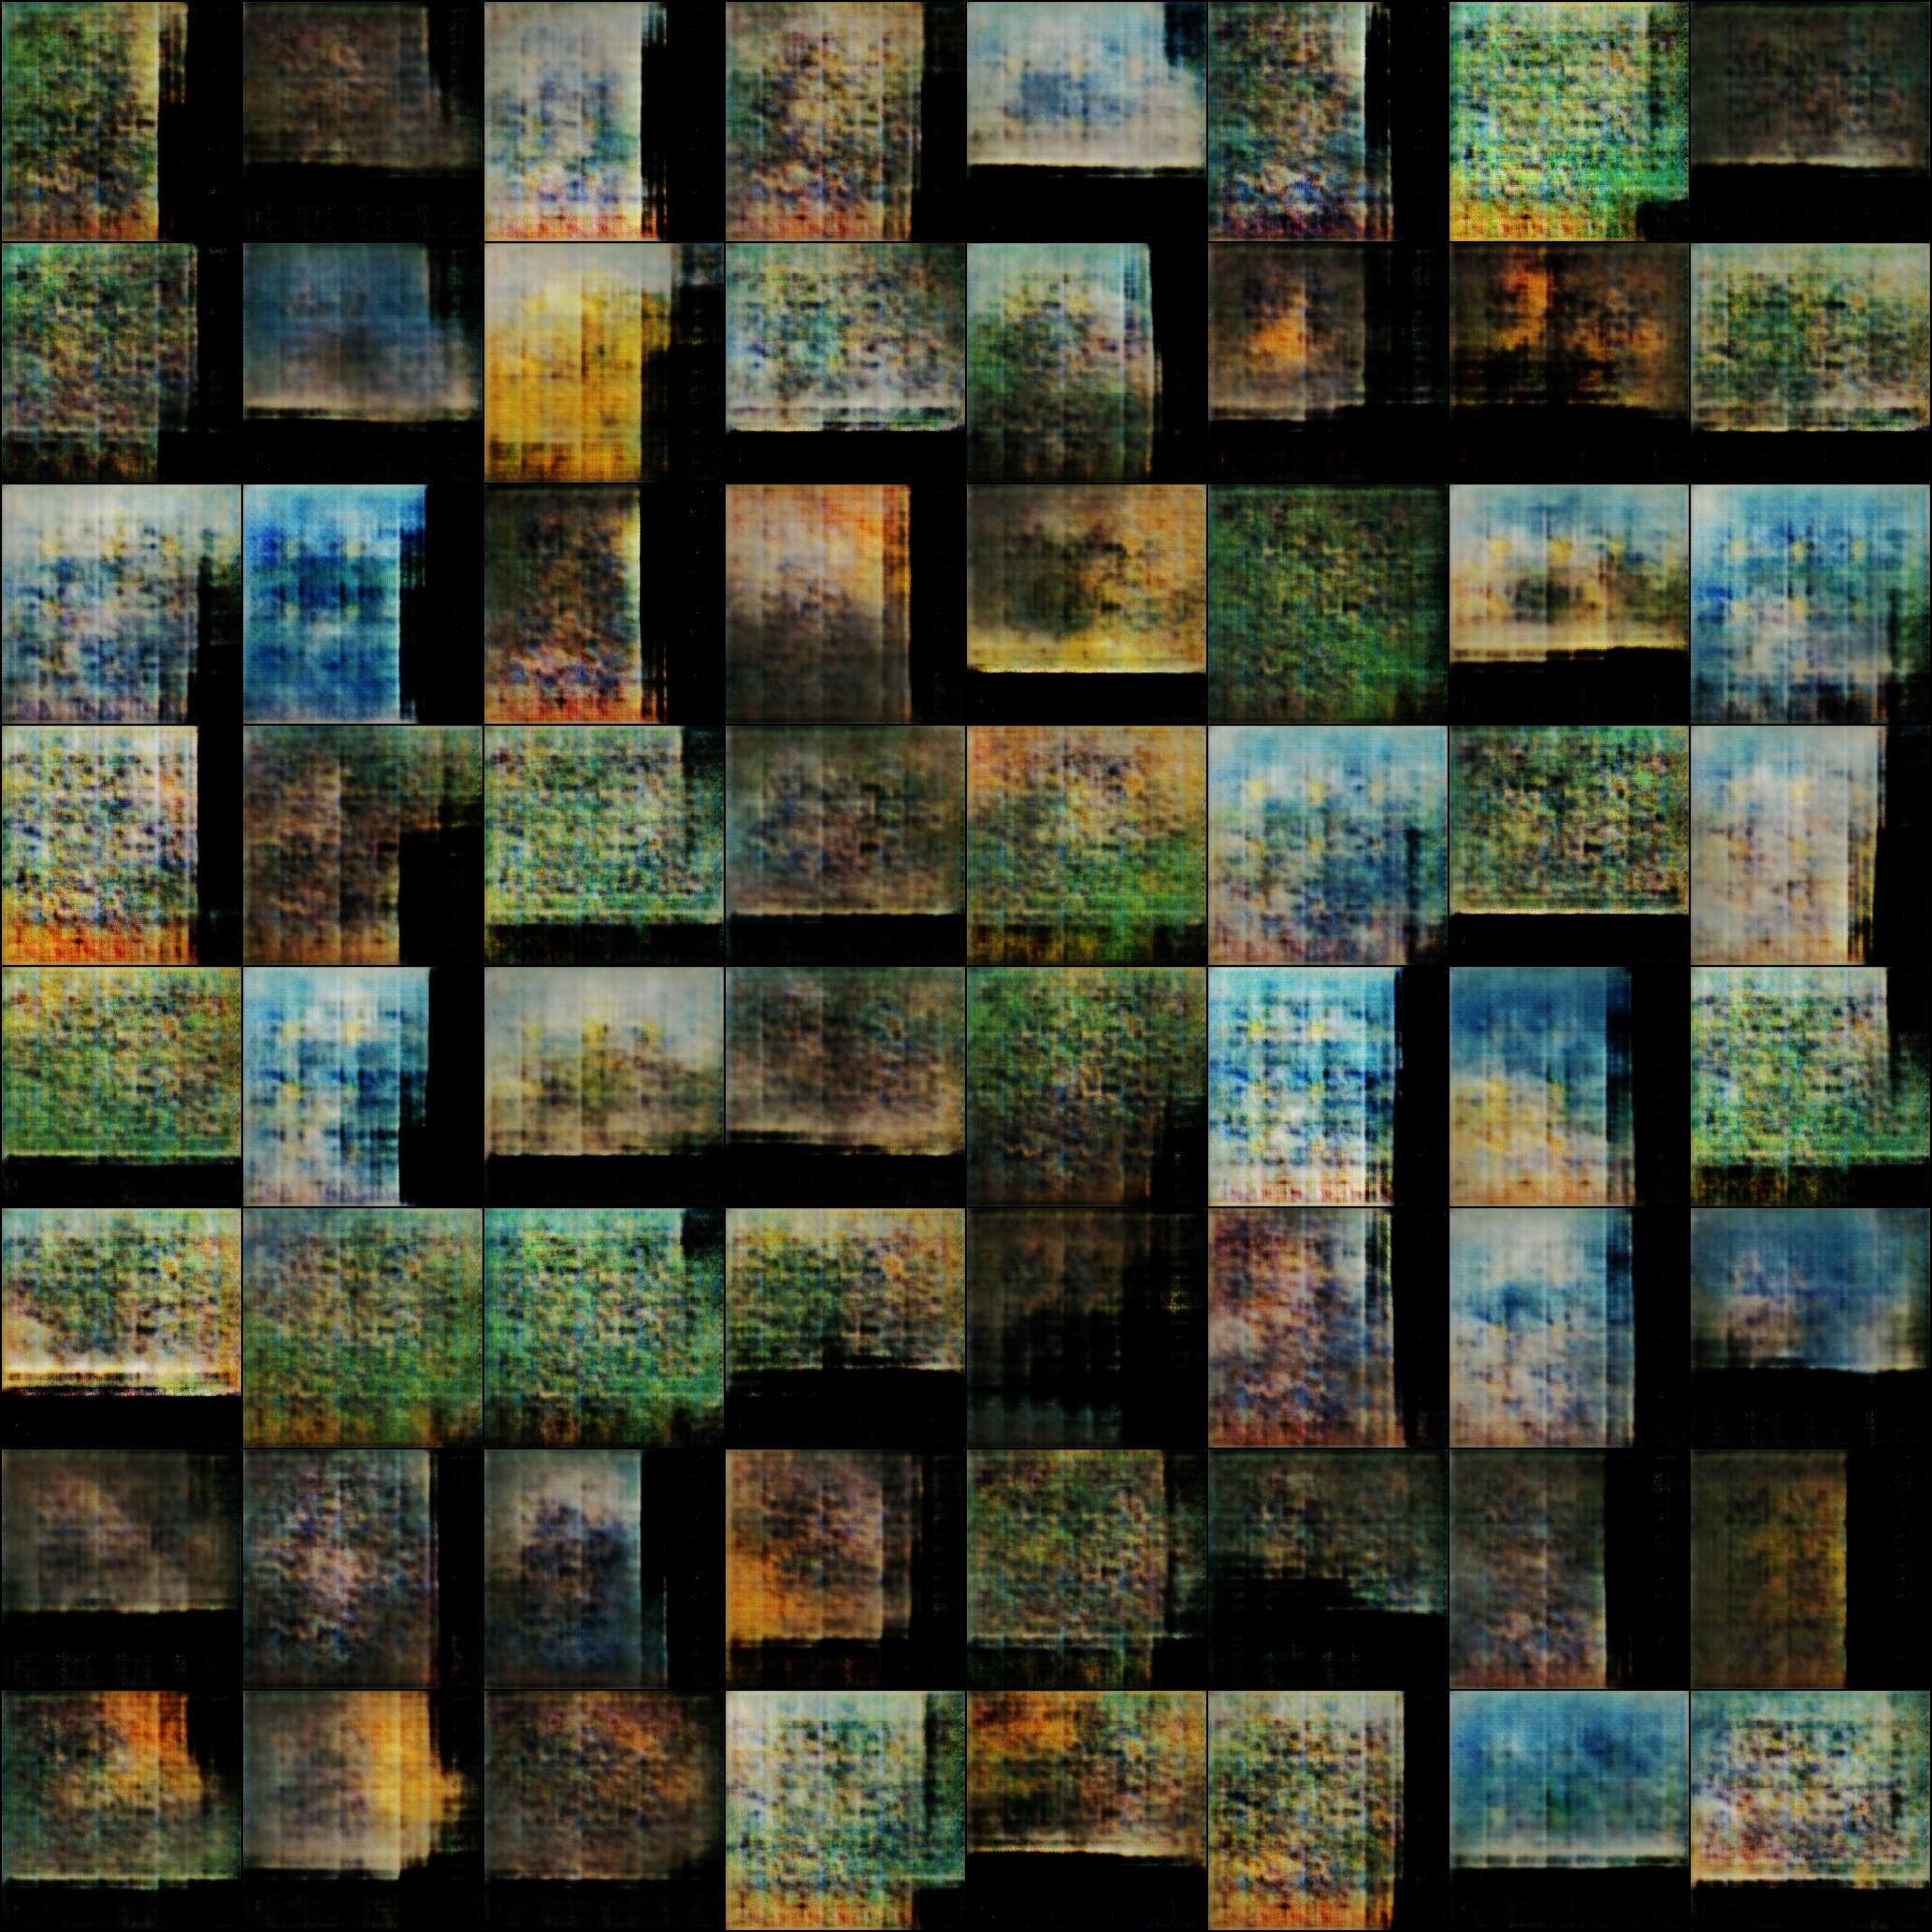
\includegraphics[width=1.0\linewidth]{past_attempts/van_gogh/DCGAN_2/images/epoch1702_generator}
					\caption[Van Gogh Museum dataset, epoch 1702]{Generated images from epoch 1702. Note that the black bars are becoming more defined.}
					\label{fig:vgm:epoch1702generator}
				\end{figure}

				At this point progress stalls for a very long time.
				It's not until around epoch 3241 that the model shows any clear progression, and even then the details are far from clearly defined.
				See figure \ref{fig:vgm:epoch3241generator}.
				\begin{figure}
					\centering
					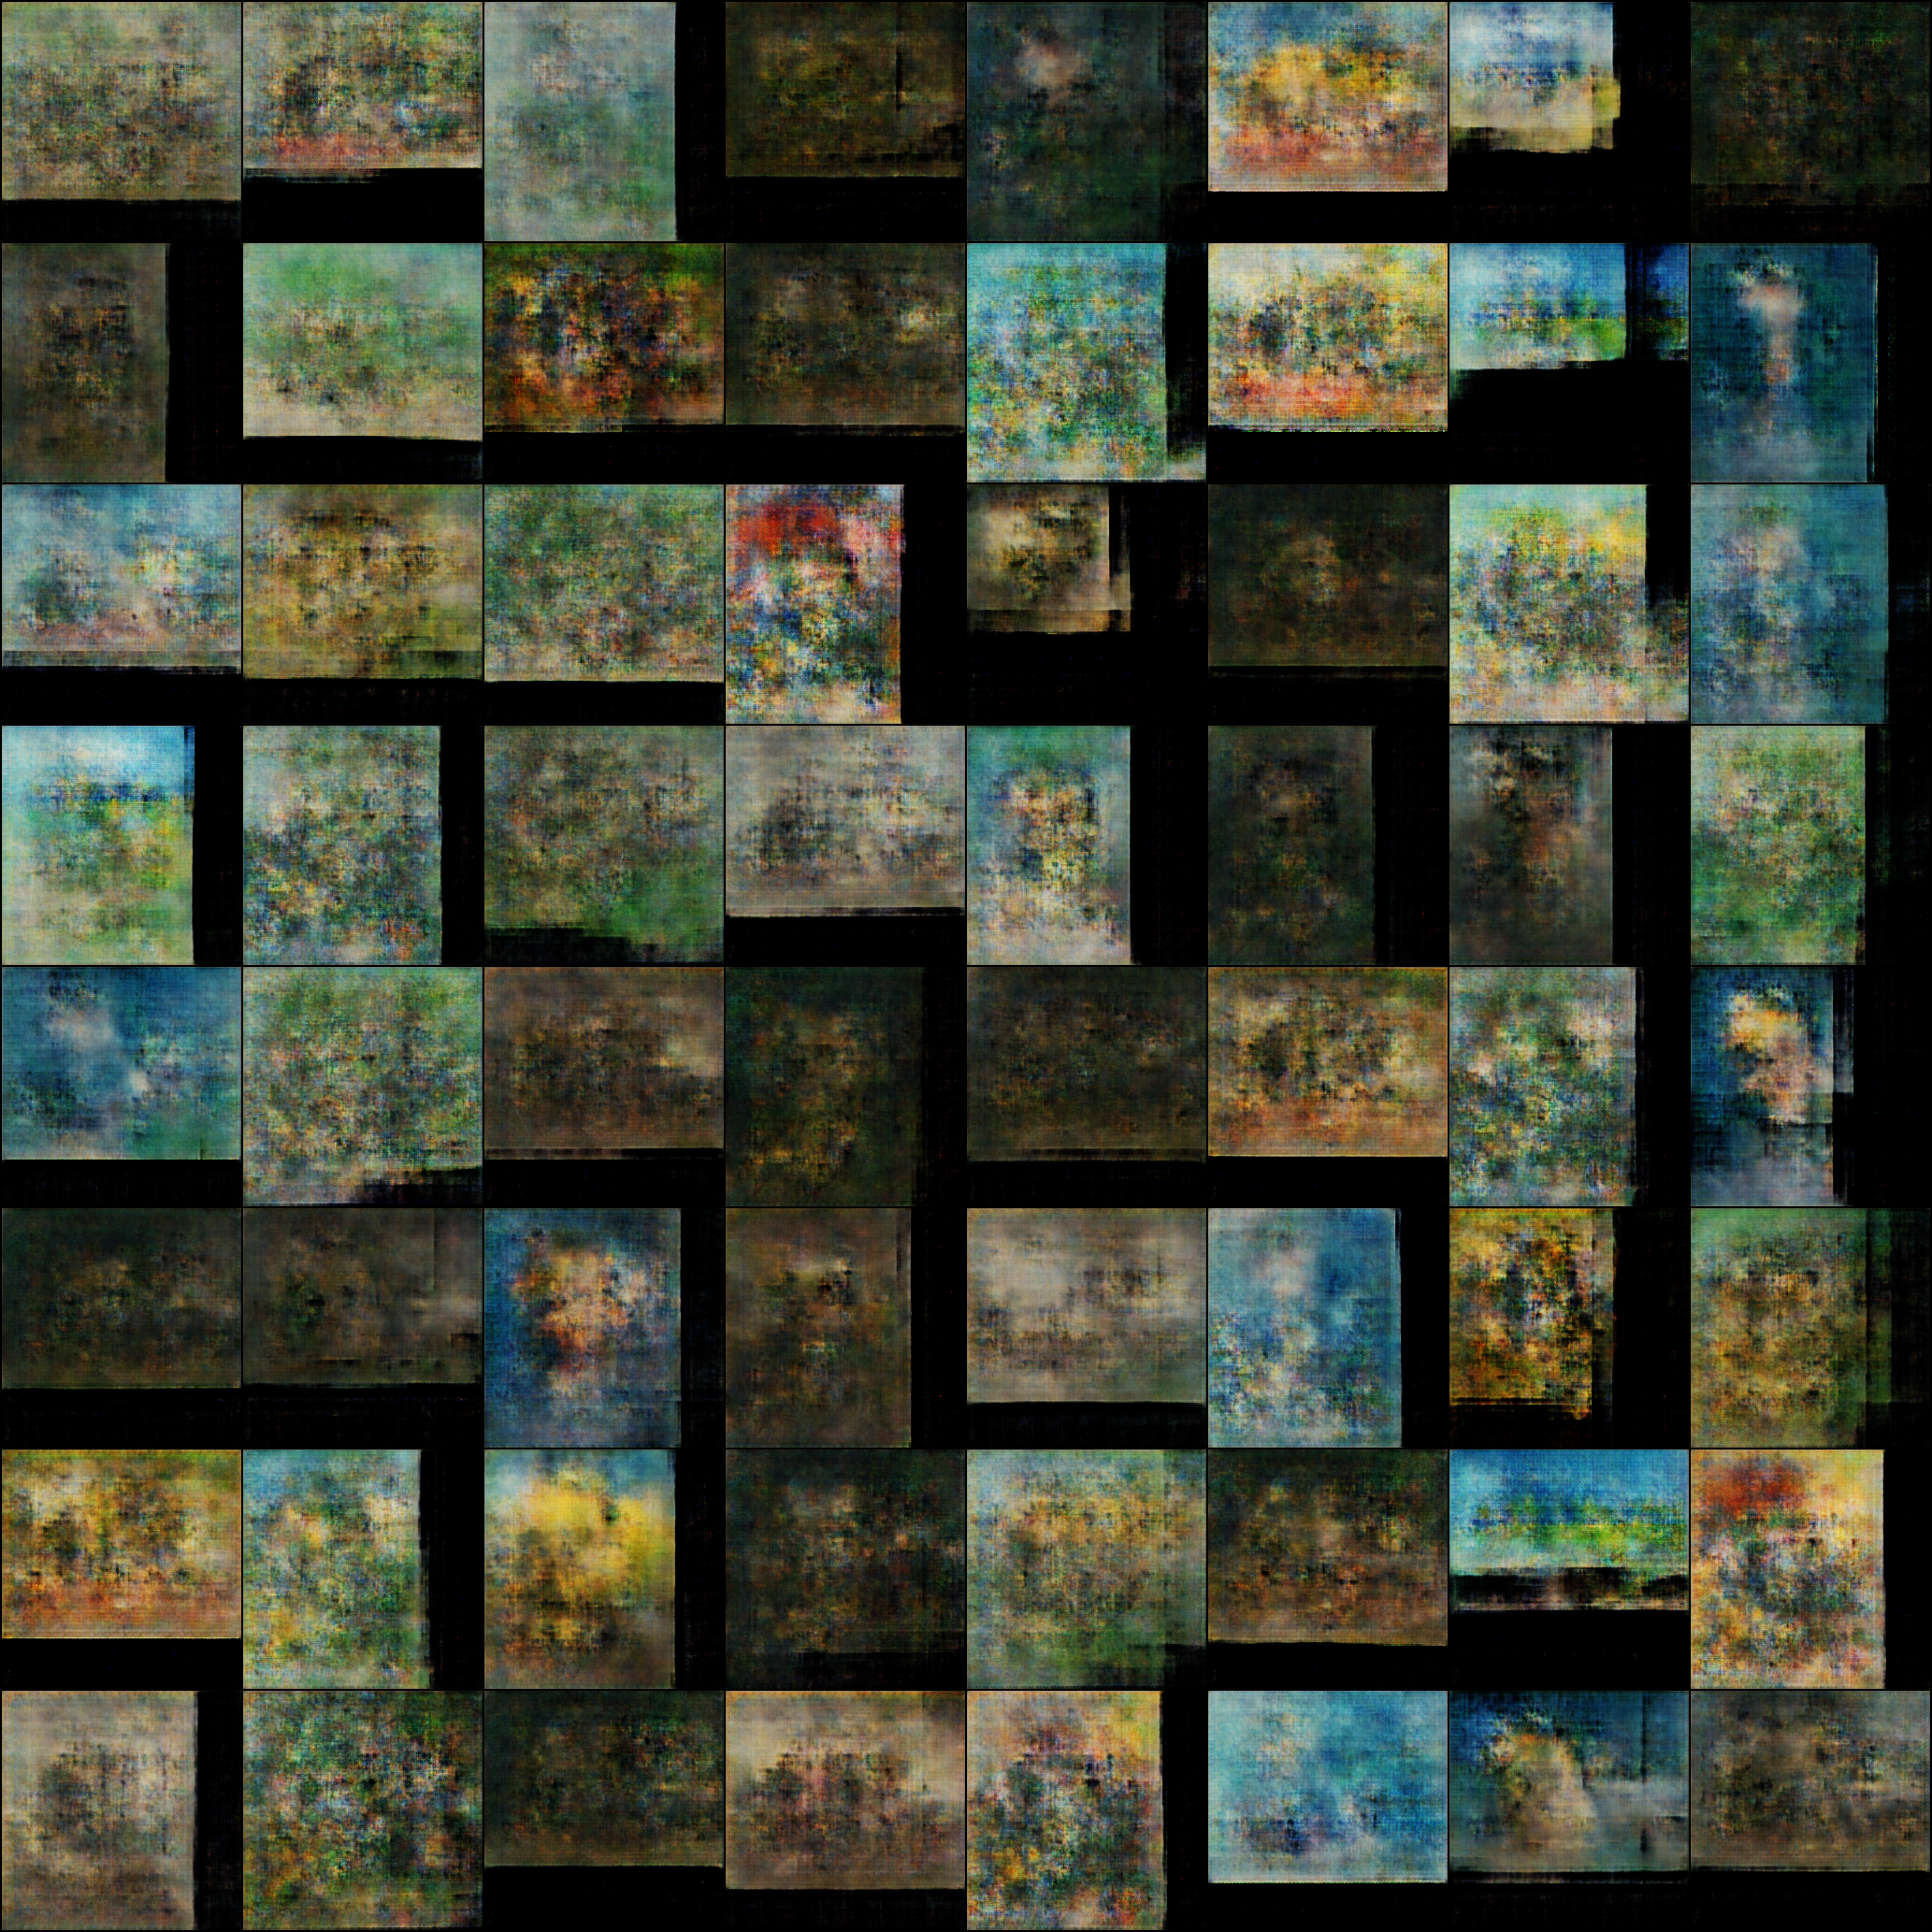
\includegraphics[width=1.0\linewidth]{past_attempts/van_gogh/DCGAN_2/images/epoch3241_generator}
					\caption[Van Gogh Museum dataset, epoch 3241]{Generated images from epoch 3241. Note the vague details forming within the images.}
					\label{fig:vgm:epoch3241generator}
				\end{figure}

				After this point, progress stops.
				Despite continuing to train the model for thousands of additional epochs, the model never achieves clearer details.
				In fact, by the final epoch, image diversity has also greatly decreased, as seen in figure \ref{fig:vgm:epoch8000generator}.
				This may suggest that the model is overfitting.
				At the very least, it is unlikely that this model would have made any further progress if we had continued to train it.
				\begin{figure}
					\centering
					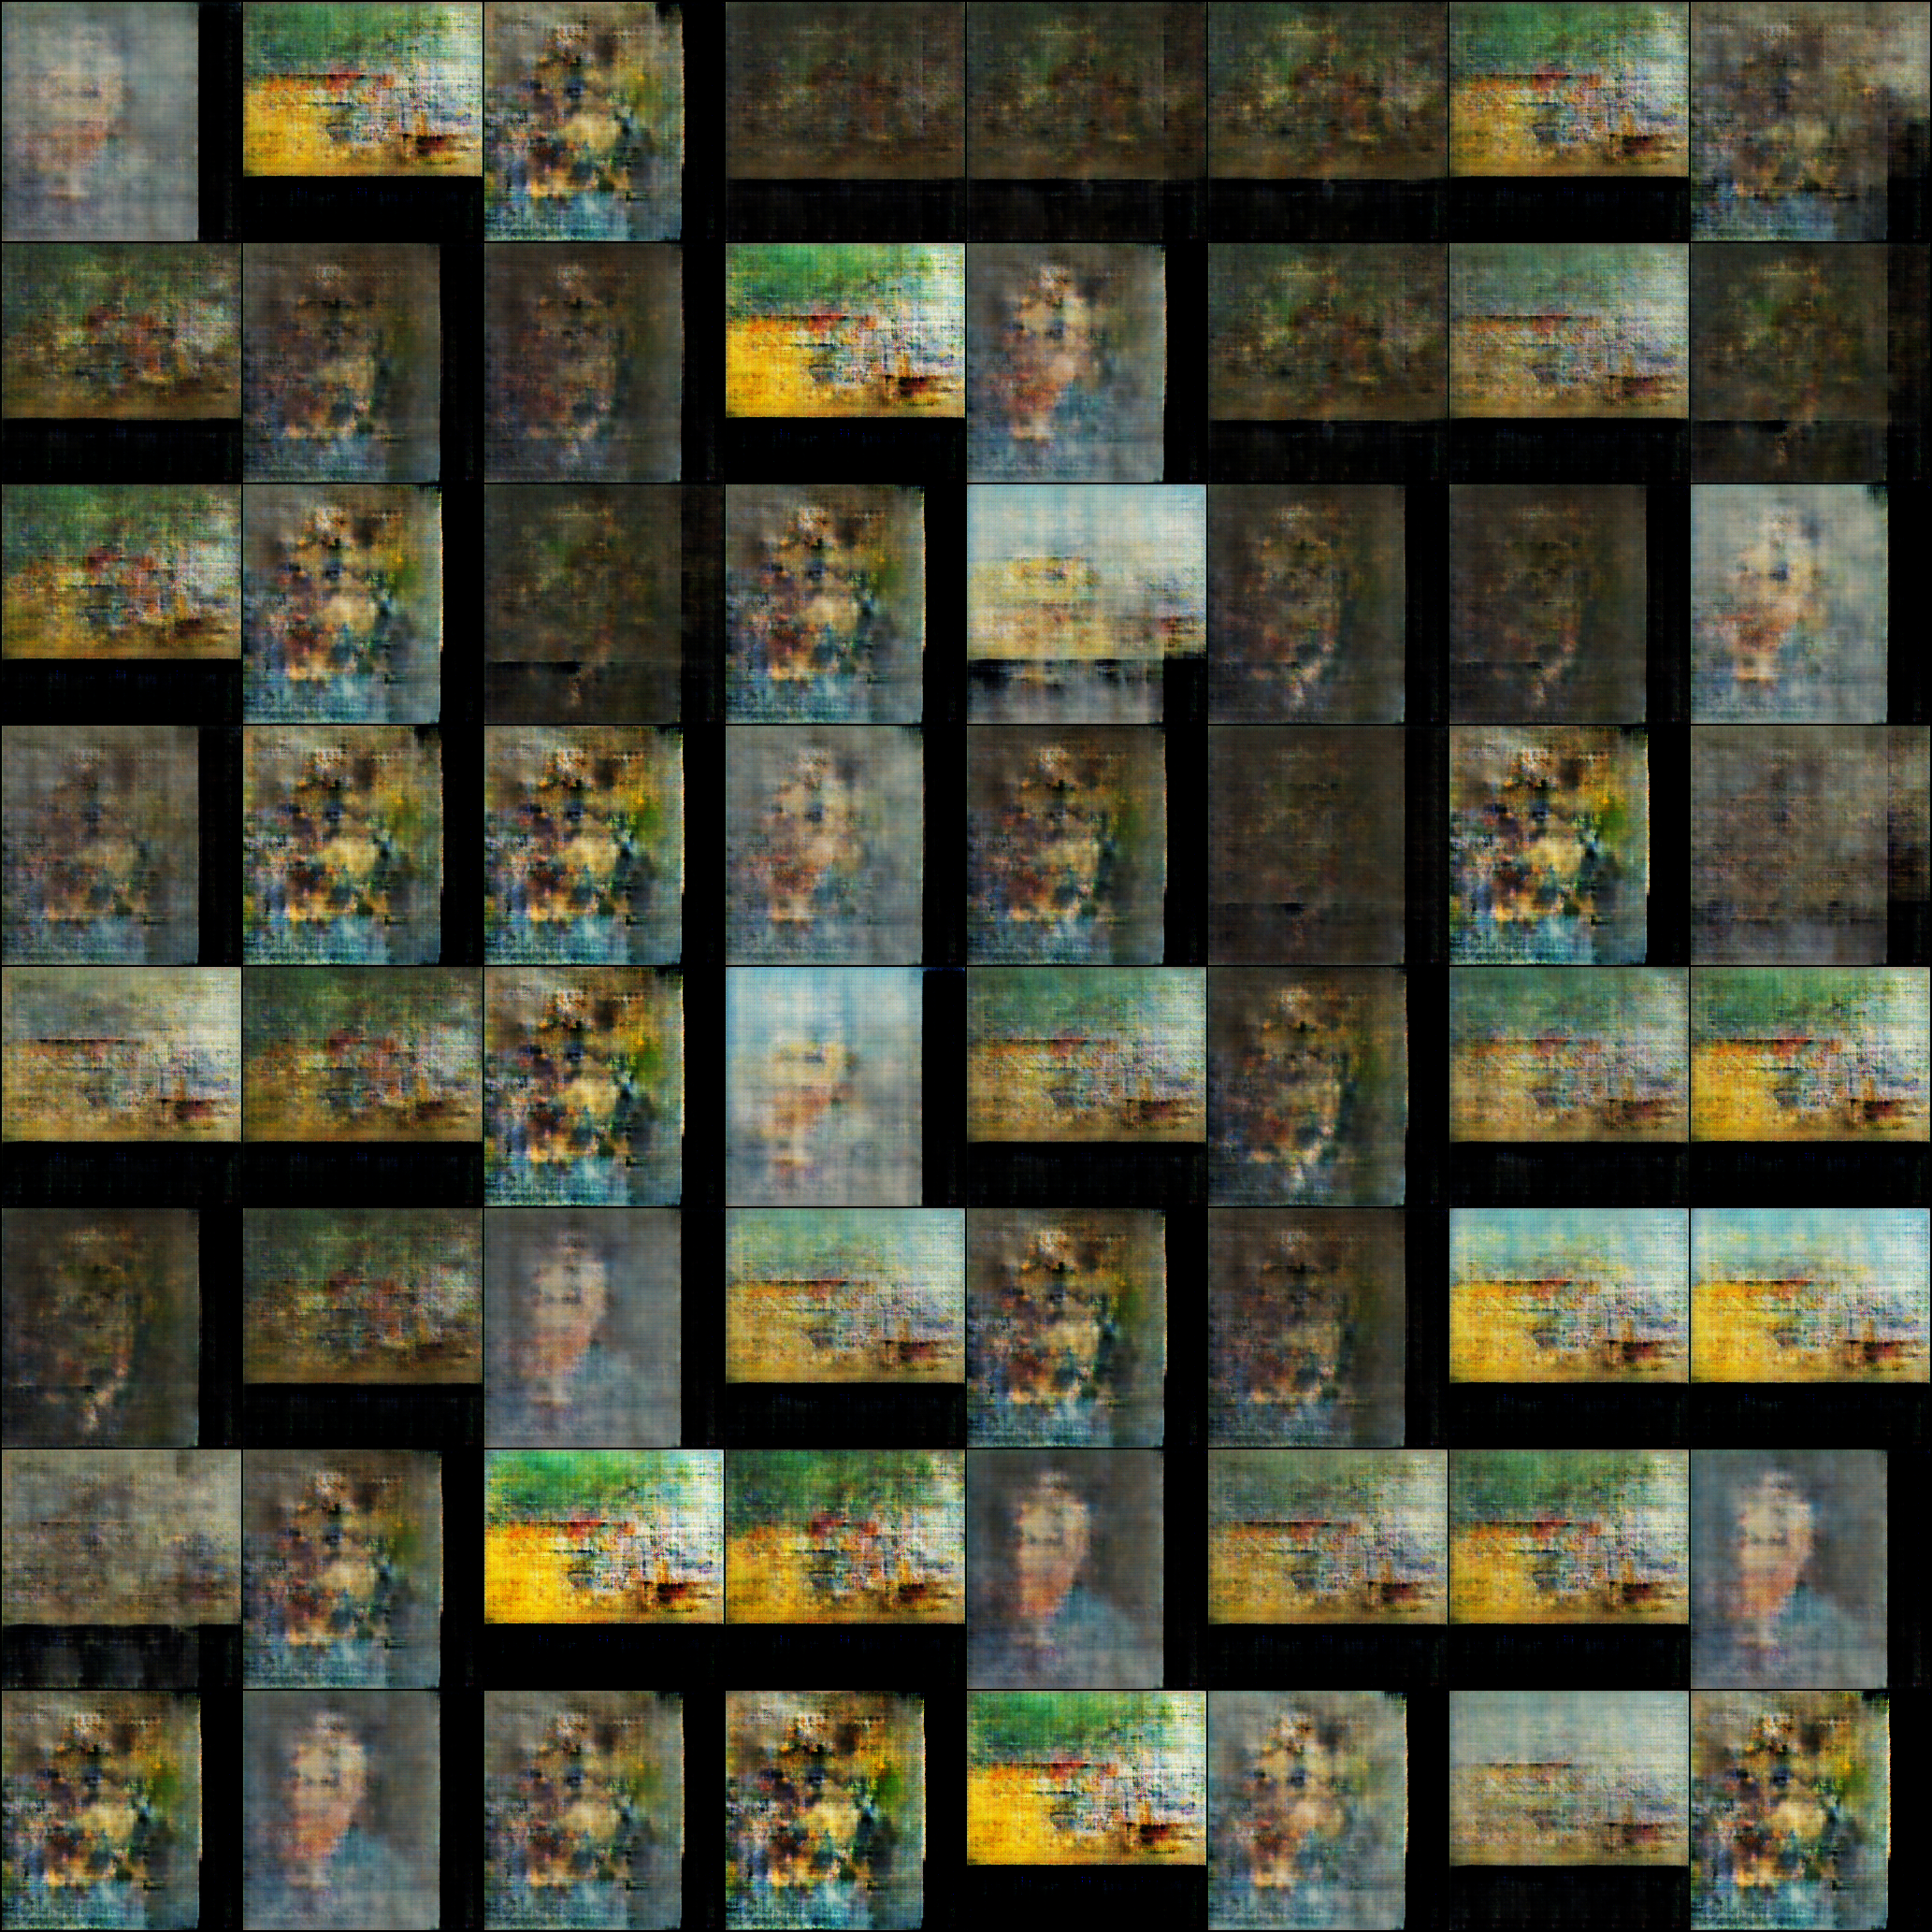
\includegraphics[width=1.0\linewidth]{past_attempts/van_gogh/DCGAN_2/images/epoch8000_generator}
					\caption[Van Gogh Museum dataset, epoch 8000]{Generated images from epoch 8000. The model has made no real progress in achieving greater clarity compared to figure \ref{fig:vgm:epoch3241generator}, and the images have become much less diverse in content.}
					\label{fig:vgm:epoch8000generator}
				\end{figure}
			\subsubsection{CycleGAN Van Gogh Dataset}


	\section{Conclusion}
		Our research has emphasized a key detail in machine learning: you need a very large dataset to get good results.
		This was shown by our models failing to converge with smaller dataset sizes.
		The datasets with 211, 400, and even 1,000 images all failed to converge.
		% failed to converge upone what
		% because they had converged to certain choices, such as color selection/ pallete
		% or horizonal deliniation (eg there's a surface (land/sea) and a sky) for the relevant data set
		
		
		The model with the smallest dataset that achieved convincing results was trained on 15,000 images.
		Future research may include determining the threshold more precisely, as there is still a large gap between 1,000 and 15,000.
		Due to this inherent limiting requirement, it seems that our initial goal of computationally determining what characteristics define Van Gogh's art was likely unattainable.

\appendix
	\section{Appendix: Weekly Progress}
		\subsection{Weeks 1-3}
		\label{subsec:weekly:1-3}
			\subsubsection{Work Completed}
				During this time period, we tested sample code from the TorchGAN\cite{pal2019torchgan} project using data from the MNIST\cite{lecun2010mnist} dataset.
				We also began writing code to provide an interface for the TorchGAN code to read from the training data we had previously collected from the Van Gogh Museum (e.g., \cite{001}, \cite{002}, \cite{003}).
			\subsubsection{Importance of Work}
				Training on the MNIST dataset demonstrated the validity of the training code.
				By verifying the results in this way, we can state with confidence that any deviation is due to the dataset, rather than the code.
			\subsubsection{Problems Encountered}
				After working on writing a subclass to use as an interface between the code and the image data, we discovered that the code was redundant, as there was a general-purpose class included in TorchGAN that could be used for that exact purpose.
				This was a setback, but ultimately allowed us to continue to move forward without having to worry about testing custom code.

		\subsection{Weeks 4-6}
			\subsubsection{Work Completed}
				This period of the project was almost entirely spent on training the model on the Van Gogh Museum dataset.
				We decided that, for the sake of reliability and availability, we would train the model locally.
			\subsubsection{Importance of Work}
				Training the model represents the bulk of the work of this project.
				While a certain amount of time has to be allocated for setting things up, the real results of the project are the models produced by training, as well as the images generated by those models.
			\subsubsection{Problems Encountered}
				Due to the hardware configuration available locally, we were not able to utilize GPU acceleration for our training.
				This meant slower training, but should not affect the quality of results, as the MNIST test was successful under the same conditions.
				Additionally, despite running the model for 8000 epochs of training, we did not achieve the expected results, and were concerned about potential overfitting.

		\subsection{Weeks 7-8}
			\subsubsection{Work Completed}
				After our first attempt did not yield results, we began looking into alternate approaches.
				While researching other GAN types that could be used, we discovered that the researchers from the CycleGAN\cite{CycleGAN2017}\cite{isola2017image} project had compiled their own Van Gogh dataset.
				The CycleGAN Van Gogh dataset consisted of 400 pictures from WikiArt\cite{wikiartVanGogh}, which was nearly twice as many images as the 211 we had been able to gather from the Van Gogh Museum.
				Additionally, the CycleGAN researchers had compiled a similar dataset of 1072 paintings by Claude Monet, also from WikiArt.
				We then began training a new model on the CycleGAN Van Gogh dataset.
			\subsubsection{Importance of Work}
				Since we knew from previous research that performance of neural networks generally improves with larger training data, these new datasets represented an unexpected opportunity to improve the quality of our results.
			\subsubsection{Problems Encountered}
				Unfortunately, even with this larger dataset, the GAN did not produce clear images.
				The color palettes of the generated images were reminiscent of a Van Gogh painting, but no clearly defined features were present.
				Any apparent features were extremely vague, and concerns about the Rorschach effect were raised.

				Additionally, since the CycleGAN dataset was nearly twice as big as the Van Gogh Museum dataset, training times increased proportionally.
				This meant that fewer epochs of training were able to be completed in the same amount of time.

		\subsection{Week 9}
			\subsubsection{Work Completed}
				At this point, we decided to try a somewhat different tactic.
				We decided to switch to the Monet dataset, and test different ways of approaching the task in order to try to figure out which might work best.
				Variables to be tested include the specific GAN being used, including both supervised and unsupervised GANs, and whether color or grayscale images would be used.
			\subsubsection{Importance of Work}
				This approach allows us to test a number of possible methods without fully committing to any of them, instead of spending all of our resources on a single variation and hoping for it to work.
				Additionally, we discovered that another, similar project had been attempted in the past\cite{otherGanGogh}, and that those researchers had encountered the same performance issues as us.
				This lends further credibility to our belief that the size of the Van Gogh datasets was simply too small for the GAN to learn from.
			\subsubsection{Problems Encountered}
				As previously noted, increasing the size of the dataset increases the time required to train the model.
				The Van Gogh Museum dataset took about 35 seconds per epoch, and the CycleGAN Van Gogh dataset took about 70.
				However, the Monet dataset takes nearly two and a half minutes per epoch, which severely limits the number of epochs that can be completed.

		\subsection{Week 10}
			\subsubsection{Work Completed}
				After speaking with our advisor this week, we decided to change focus once again.
				Our current goal is to attempt to replicate the results of the other GANGogh project \cite{otherGanGogh}.
				We are training a model on the dataset of landscape paintings that Jones and Bonafilia compiled from WikiArt.
				This has so far been much more successful than previous attempts with other datasets.
			\subsubsection{Importance of Work}
				If we are able to reproduce the results of Jones and Bonafilia, it will further confirm that the problems we encountered with the Van Gogh datasets was due to their size.
			\subsubsection{Problems Encountered}
				At 15,000 images, the landscapes dataset is much larger than any of our previous datasets, with the sole exception of the MNIST dataset.
				Despite reducing the size of the training images to 64 by 64 pixels, this dataset still takes between 5 and 15 minutes\footnote{Most epochs take 5 minutes, but occasionally one will take two or three times that long, presumably due to other applications running at the same time. This is, however, a much greater variance than has been observed with other datasets, even under the same conditions.} per epoch of training.
				However, unlike previous time-consuming training attempts, this one appears to be making significant progress.
				The small size of the images limits the amount of detail that can be shown, but after 400 epochs, the model is consistently producing convincing images.

		\subsection{Weeks 11-13}
			\subsubsection{Work Completed}
				After successfully reproducing the results of Jones and Bonafilia at a resolution of 64 by 64 pixels, we attempted the same task, but at a resolution of 128 by 128 pixels.

			\subsubsection{Importance of Work}
				While the 64 by 64 images were convincingly similar to the original images resized to that resolution, the small size limits the amount of detail able to be shown.
				The ability to generate similarly convincing, larger images confirms that the GAN is actually learning the patterns that we want it to be learning.

			\subsubsection{Problems Encountered}
				As expected, increasing the resolution increased the length of each epoch of training.
				At 128 by 128 pixels, each epoch takes 10 to 20 minutes.
				Additionally, despite our success with the smaller resolution at 400 epochs, the same number of epochs have not produced the same level of results with this model.
				At 700 epochs, the model is able to produce some convincing images, but not nearly as consistently as the previous model.


\bibliographystyle{IEEEtran}
\bibliography{van_gogh_bib}
\nocite{*}
\end{document}
